\documentclass[11pt,a4paper]{report}

\usepackage[utf8]{inputenc}
\usepackage[T1]{fontenc}

\pagestyle{empty}

\usepackage{graphicx} % Include figure files
\usepackage{amstext,amsbsy,amssymb}
\usepackage{amsmath}
%\usepackage{times} 

%% Numbered problems
\newcounter{excount}[chapter]
\newenvironment{exercise}[1][]{\addtocounter{excount}{1} \noindent {\bf Problem
    \arabic{excount} \ \ #1}\hspace{2mm}}{\vspace{4mm}}


\title{FYS3120 Classical Mechanics and Electrodynamics\\ 
\vspace{15mm}Problem set 9}


%%%%%%%
\begin{document}
%%%%%%%
\maketitle


%%%%%%%%%%
\begin{exercise}
%%%%%%%%%%
Two photons in the laboratory system have frequencies $\nu_1$ and $\nu_2$. The angle between their propagation directions is $\theta$.
\begin{itemize}
\item[\bf a)] Find the total energy and the absolute value of the total momentum of the photons in the laboratory system, expressed in terms of the frequencies $\nu_1$ and $\nu_2$.
\item $E=h(\nu_1+\nu_2)$
\item $\vec{P}_1=(E_1/c,\vec{p_1})=p_1(1,1,0,0)=\frac{h}{c}\nu_1(1,1,0,0), \vec{P}_2=(E_2/c,\vec{p_2})=\frac{h}{c}\nu_2(1,\cos \theta,\sin \theta,0)$. $|p|=|\vec{p}_1+\vec{p}_2|=|\frac{h}{c} (\nu_1+\nu_2 \cos \theta,\nu_2 sin \theta)|=\frac{h}{c}\sqrt{(\nu_1+\nu_2\cos \theta)^2+\nu_2^2\sin^2 \theta}=\frac{h}{c}(\nu_1^2+2\nu_1\nu_2 \cos \theta + \nu_2^2)$
\item[\bf b)] Find the photons' frequency in the center-of-mass system.
\item Minkowski norm squared of 4mom: $P\mu P\mu=|\vec{p}|^2-\frac{E^2}{c^2}$ is Lorentz invariant. Thus: $\frac{h}{c}(\nu_1^2+2\nu_1\nu_2 \cos \theta + \nu_2^2)=-\frac{E'}{c}$, where $E'$ is the energy of the photons in the center-of-mass system $|p|=0$, defined by $\sum_k \vec{p}=0$. $\sum_k \vec{p}=0 \implies \nu_1'=\nu_2'=\nu' \implies E'=2\frac{h}{c}\nu' \implies \nu'=\nu_1^2+2\nu_1\nu_2 \cos \theta + \nu_2^2$
\item[\bf c)] Is it always possible to find a center-of-mass system for the photons?
\item No. If the angle of propagation is is zero,it would not be possible to find a center-of-mass system for the photons. 
\end{itemize}
\end{exercise}


%%%%%%%%%%
\begin{exercise}
%%%%%%%%%%
We send a photon $\gamma$ towards an electron $e^-$ at rest.
\begin{itemize}
\item[\bf a)] What is the minimum energy of the photon required for the following process to take place
\begin{equation}
\gamma + e^- \rightarrow e^- + e^- + e^+ \ \text{?   }
\end{equation}
The particles $e^-$ and $e^+$ have the same mass $m_e$.
\item After having done some brief reading on pair production my understanding is that the photon must have higher energy than the rest masses of the produced electron and proton. My guess is that electron positron annihilation happens unless the two new particles are spaced appart, but I really don't know. Anyway, applying energy conservation:
$E_{\gamma}+E_-=2E_-+E_+ +E_R \implies  E_{\gamma}=2m_ec^2 +E_R$. Assuming that any residual energy is sufficient, $E_{\gamma}>2m_ec^2$ or $E_{\gamma}> 1.022 MeV$
\item[\bf b)] Show that the process
\begin{equation}
\gamma \rightarrow e^- + e^+,
\end{equation}
is impossible.
\item Energy conservation: $E_{\gamma}=E_-+E_+$ 
\item Subsituting the relativistic energy-momentum relation $E^2=c^2p^2+m^2c^4$ into the energy conservation: 
$E_{\gamma}=\sqrt{p_{\gamma}^2c^2}=p_{\gamma}c=\sqrt{p_-^2c^2+m_e^2}+\sqrt{p_+^2c^2+m_e^2}$. 
\item Momentum conservation: $P_{\gamma}=P_                                                                                                                                                                                                                                                                                                                                                                     -+P_+ \implies p_{\gamma}c=p_-c+p_+c$. Comparing this with the expression above derived from energy conservation leads to the conclusion that the process is impossible.
\end{itemize}
\end{exercise}


%%%%%%%%%%
\begin{exercise}[Exam 2005]\\
%%%%%%%%%%
A photon with energy  $E_f=100\,\text{keV}$ is scattered on a free electron, which is, before the scattering, at rest in the laboratory frame. After the scattering the energy of the photon is  $E'_f$, and the direction of propagation makes an angle $\theta$ relative to the direction of the incoming photon. The rest energy of the electron is $E_e=m_e c^2=0.511\,\text{MeV}$, and after the scattering it has an energy which we denote by  $E'_e$. The electron is scattered in a direction which makes an angle   $\chi$ relative to the direction of the incoming photon. 

%%%%%%%%%%%%
\begin{figure}[h]
\begin{center}
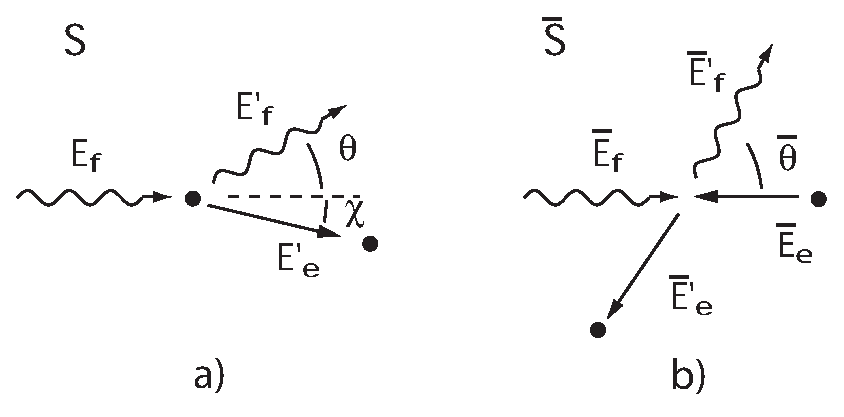
\includegraphics[height=4cm]{Compton.eps}
\caption{Compton scattering in a) the lab frame, b) in the centre-of-mass system.}
\label{fig:compton}
\end{center}
\end{figure}
%%%%%%%%%%%%

We examine this process both in the lab frame $S$ (Fig.~\ref{fig:compton}a) and in the center of mass system $\bar S$ (Fig.~\ref{fig:compton}b). In order to keep track,  in the center of mass system all variables are marked with a ``bar'', for example $\bar E_f$ for the energy of the incoming photon.

\begin{itemize}
\item[\bf a)] What is meant by the center-of-mass system? Use the transformation formulas for energy and momentum to determine the relative velocity between the lab system and the center-of-mass system.
\item In relativistic physics, the center-of-mass system is the system in which the space part of the four-vectors of the system is zero: $\sum_k \mathbf{p}_k=0$
\item Momentum transformation for the photon: $\bar{p_f}^1 c=\bar{p_f}c=\gamma(p_f^1-\beta p_f^0)=\gamma(1-\beta)p_f$, where $p_f=E_f/c$
\item From the definition of the center-of-mass system, it follows that: $\bar{p_f}=-\bar{p_e}$, thus: $-\bar{p_e}=-\gamma m_e \bar{v_e}=\gamma(1-\beta)p_f \implies -\bar{v_e}=(1-\beta)p_f/m_e=(1-v^2/c^2)\frac{E_f}{c m_e } \implies \frac{E_f}{c m_e } \frac{1}{c^2} v^2 - \bar{v_e} -\frac{E_f}{c m_e }=0$, as $v_e=0$, $v=-\bar{v_e}$ is the relative velocity between the lab system and the center-of-mass system, so: $\frac{E_f}{c m_e } \frac{1}{c^2} v^2 +v -\frac{E_f}{c m_e }=\frac{E_f}{E_e} \frac{1}{c} v^2 +v -\frac{E_f}{E_e}c=0 \implies v=\frac{-1\pm \sqrt{1+4\frac{E_f}{E_e}\frac{E_f}{E_e}}}{\frac{E_f}{E_e}} c$, taking $v>0 \implies v\approx0.477c$. \textit{Intuitively, I would expect a smaller velocity. This either indicates that my intuition is wrong, or that that my calculation is wrong, and I'm not sure which worse.}


\item[\bf b)] Explain why the energy of the incoming and outgoing photon is the same in the center-of-mass system and find this energy.
\item I was not able to figure out a good explaination, although I understand that this might be the case, as any change in photon momentum is reflected in a change of rest frame. I was however not able to show this in any way. 
\item[\bf c)] If $\theta=90^{\circ}$ what is the energy of the outgoing photon in the lab system? What is the corresponding energy of the outgoing electron?
Using the Compton Formula:
$\lambda'-\lambda=\frac{h}{m_ec}(1-cos \theta), \theta=90 \implies \frac{c}{E'}-\frac{c}{E}=\frac{1}{m_e c} \implies E'=\frac{1}{\frac{1}{m_e c^2}+\frac{1}{E}}\approx 86.3$ keV, which intuitively makes sense. Collision has transfered some energy to the electron.
\end{itemize}
\end{exercise}


%%%%%%%%%%
\end{document}
%%%%%%%%%%


